\documentclass{article}

\usepackage{amsmath, amssymb}
\usepackage{multicol}
\usepackage[table]{xcolor}
\usepackage{forest}
\usepackage[a4paper, bindingoffset=0in, left=0.2in, right=0.1in, top=0.15in,
            bottom=0.2in, footskip=0.25in]{geometry}
\usepackage{parskip}
\usepackage{draftwatermark}
\usepackage{enumitem}
\usepackage{multicol}
\usepackage{makecell}	
\usepackage{listings}

\SetWatermarkColor[gray]{0.95} \SetWatermarkText{Isaac Boaz}
\SetWatermarkScale{1}

\pagenumbering{gobble}

\begin{document}
\small

\setlist{nosep}
\setlength{\parindent}{0em}
\setlength{\itemindent}{0em}
\setlength{\leftmargini}{0em}

\begin{multicols*}{2}
    \subsection*{General DP Remarks}
    \subsubsection*{Optimal Substructure}
    \begin{itemize}
        \item Create optimal solution to problem using optimal solutions to
              subproblems.
        \item Can't use DP if optimal solution to a problem does not require
              subproblem solutions to be optimal. \\
              \(\rightarrow\) Often happens when subproblems are \emph{not
                  independent} of each other.
    \end{itemize}
    \subsubsection*{Overlapping Subproblems}
    \begin{itemize}
        \item For DP to be useful, recursive algorithm should require us to
              compute optimal solutions to the \emph{same subproblems} over and
              over again.
        \item In total, there should be a small number of distinct subproblems
              (i.e. polynomial in input size).
    \end{itemize}

    \subsection*{LCS}
    \begin{equation*}
        LCS[i, j] = \begin{cases}
            0                              & \text{if } i = 0 \text{ or } j = 0 \\
            1 + LCS[i-1, j-1]              & \text{if } x_i = y_i               \\
            \max(LCS[i-1, j], LCS[i, j-1]) & \text{otherwise}
        \end{cases}
    \end{equation*}
    \hspace*{-1.5em}
    \begin{tabular}{|c|c|c|c|c|c|c|c|c|c|c|}
        \hline
                                       &                               & j=0 &
        j=1                            & j=2
                                       & j=3                           & j=4 &
        j=5                            & j=6
                                       & j=7                           & j=8     \\
        \hline
                                       &                               &     & p
                                       & r                             & i   & n
                                       & t                             & i   & n
                                       & g                                       \\
        \hline
        i=0                            &                               & 0   & 0
                                       & 0                             & 0   & 0
                                       & 0                             & 0   & 0
                                       & 0                                       \\
        \hline
        i=1                            & s                             & 0   & 0
                                       & 0                             & 0   & 0
                                       & 0                             & 0   & 0
                                       & 0                                       \\
        \hline
        i=2                            & p                             & 0   &
        \cellcolor{red!25} 1$\nwarrow$ &
        1$\leftarrow$                  &
        1$\leftarrow$                  & 1$\leftarrow$
                                       & 1$\leftarrow$                 &
        1$\leftarrow$                  &
        1$\leftarrow$                  &
        1$\leftarrow$                                                            \\
        \hline
        i=3                            & r                             & 0   &
        1$\uparrow$                    &
        \cellcolor{red!25} 2$\nwarrow$ &
        2$\leftarrow$                  &
        2$\leftarrow$                  &
        2$\leftarrow$                  & 2$\leftarrow$
                                       & 2$\leftarrow$                 &
        2$\leftarrow$                                                            \\
        \hline
        i=4                            & i                             & 0   &
        1$\uparrow$                    &
        2$\uparrow$                    &
        \cellcolor{red!25}3$\nwarrow$  &
        3$\leftarrow$                  &
        3$\leftarrow$                  &
        3$\leftarrow$                  &
        3$\leftarrow$                  &
        3$\leftarrow$                                                            \\
        \hline
        i=5                            & n                             & 0   &
        1$\uparrow$                    &
        2$\uparrow$                    &
        3$\uparrow$                    &
        \cellcolor{red!25}4$\nwarrow$  &
        4$\leftarrow$                  &
        4$\leftarrow$                  &
        4$\leftarrow$                  &
        4$\leftarrow$                                                            \\
        \hline
        i=6                            & g                             & 0   &
        1$\uparrow$                    &
        2$\uparrow$                    &
        3$\uparrow$                    & 4$\uparrow$
                                       & 4$\uparrow$                   &
        4$\uparrow$                    &
        4$\uparrow$                    &
        5$\nwarrow$                                                              \\
        \hline
        i=7                            & t                             & 0   &
        1$\uparrow$                    &
        2$\uparrow$                    &
        3$\uparrow$                    & 4$\uparrow$
                                       & \cellcolor{red!25}5$\nwarrow$ &
        5$\leftarrow$                  &
        5$\leftarrow$                  &
        5$\leftarrow$                                                            \\
        \hline
        i=8                            & i                             & 0   &
        1$\uparrow$                    &
        2$\uparrow$                    &
        3$\nwarrow$                    & 4$\uparrow$
                                       & 5$\uparrow$                   &
        \cellcolor{red!25}6$\nwarrow$  &
        6$\leftarrow$                  &
        6$\leftarrow$                                                            \\
        \hline
        i=9                            & m                             & 0   &
        1$\uparrow$                    &
        2$\uparrow$                    &
        3$\uparrow$                    & 4$\uparrow$
                                       & 5$\uparrow$                   &
        6$\uparrow$                    &
        6$\uparrow$                    &
        6$\uparrow$                                                              \\
        \hline
        i=10                           & e                             & 0   &
        1$\uparrow$                    &
        2$\uparrow$                    &
        3$\uparrow$                    & 4$\uparrow$
                                       & 5$\uparrow$                   &
        6$\uparrow$                    &
        6$\uparrow$                    &
        6$\uparrow$                                                              \\
        \hline
    \end{tabular}

    \subsection*{OBST}
    \begin{itemize}
        \item Any subtree of a BST contains keys in a contiguous range \(k_i,
              \ldots, k_j\) for some \(1 \leq i \leq j \leq n\).
        \item If \(T\) is an OBST, and \(T\) contains subtree \(T'\) with keys
              \(k_i, \ldots, k_j\), then \(T'\) must be an OBST for keys \(k_i,
              \ldots, k_j\).
        \item Examine all candidate roots \(k_r\) for \(i \leq r \leq j\).
        \item Determine all OBSTs containing \(k_i, \ldots, k_{r-1}\) and
              containing \(k_{r+1}, \ldots, k_j\)
    \end{itemize}
    \begin{equation*}
        e[i, j] = \begin{cases}
            0                                                          & \text{if } i = j - 1 \\
            \min_{i \leq r \leq j} \{e[i, r-1] + e[r+1, j] + w(i, j)\} & \text{if } i \leq j
        \end{cases}
    \end{equation*}
    \begin{equation*}
        root[i, j] = \text{root of subtree with keys } k_i, \ldots, k_j \text{ for } 1 \leq i \leq j \leq n
    \end{equation*}
    \begin{align*}
        w[1, \ldots & , n+1, 0, \ldots, n]  = \text{ sum of probabilities}          \\
                    & w[i, i-1] = 0 \text{ for } 1 \leq i \leq n                    \\
                    & w[i, j] = w[i, j-1] + p_j \text{ for } 1 \leq i \leq j \leq n
    \end{align*}

    Consider 5 keys with search probabilities \(p_1 = 0.25, p_2 = 0.2, p_3 =
    0.05, p_4 = 0.2, p_5 = 0.3\)

    \hspace*{-1.5em}
    \setlength\tabcolsep{2.5pt}
    % \footnotesize
    \begin{multicols}{2}
        \begin{center}
            \begin{tabular}{c|cccccc}
                w & 0 & 1    & 2    & 3    & 4    & 5    \\
                \hline
                1 & 0 & 0.25 & 0.45 & 0.5  & 0.7  & 1.0  \\
                2 &   & 0    & 0.2  & 0.25 & 0.45 & 0.55 \\
                3 &   &      & 0    & 0.05 & 0.25 & 0.55 \\
                4 &   &      &      & 0    & 0.2  & 0.5  \\
                5 &   &      &      &      & 0    & 0.3  \\
                6 &   &      &      &      &      & 0    \\
                \\
                % \end{tabular} \\
                % \begin{tabular}{c|cccccc}
                r & 0 & 1    & 2    & 3    & 4    & 5    \\
                \hline
                1 &   & 1    & 1    & 1    & 2    & 2    \\
                2 &   &      & 2    & 2    & 2    & 4    \\
                3 &   &      &      & 3    & 4    & 5    \\
                4 &   &      &      &      & 4    & 5    \\
                5 &   &      &      &      &      & 5    \\
                6 &   &      &      &      &      &      \\
            \end{tabular}
        \end{center}
        \columnbreak
        \begin{center}
            \begin{tabular}{c|cccccc}
                e & 0 & 1    & 2    & 3    & 4    & 5    \\
                \hline
                1 & 0 & 0.25 & 0.65 & 0.8  & 1.25 & 2.1  \\
                2 &   & 0    & 0.2  & 0.3  & 0.75 & 1.35 \\
                3 &   &      & 0    & 0.05 & 0.3  & 0.85 \\
                4 &   &      &      & 0    & 0.2  & 0.7  \\
                5 &   &      &      &      & 0    & 0.3  \\
                6 &   &      &      &      &      & 0    \\
            \end{tabular}

            \begin{forest}
                [\(k_2\) [\(k_1\)] [\(k_5\) [\(k_4\) [\(k_3\)] [, phantom] ] [,
                                    phantom] ] ]
            \end{forest}
        \end{center}
    \end{multicols}
    \small

    \subsection*{DFS}
    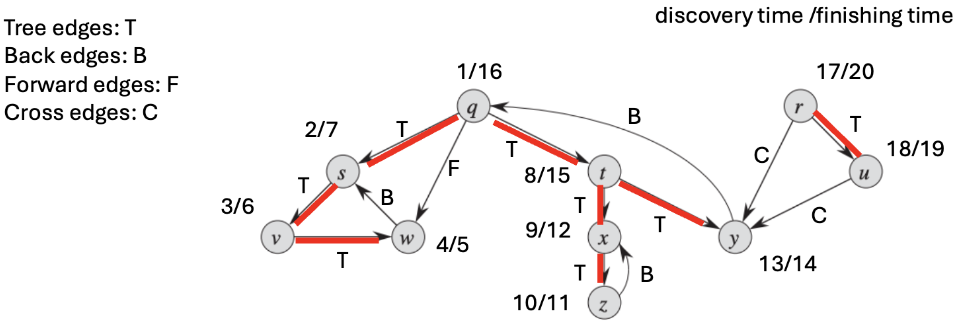
\includegraphics[width=\linewidth]{dfs.png}
    % \vspace{-3em}
    \begin{equation*}
        \left(q\left[s\{v(ww)v\}s\right][t\{x(zz)x\}yyt]q\right)(r[uu]r)
    \end{equation*}
    \begin{description}
        \item[Tree Edges] Are edges in depth-first forest \(G_\pi\). Edge \((u,
            v)\) is a tree edge if $v$ was first discovered by exploring edge
            \((u, v)\)
        \item[Back Edges] Are edges \((u, v)\) connecting a vertex $u$ to an
            ancestor in a depth-first tree. We consider self-loops, which may
            occur in directed graphs, to be back edges.
        \item[Forward Edges] Are nontree edges \((u, v)\) connecting a vertex
            $u$ to a descendant $v$ in a depth-first tree.
        \item[Cross Edges] Are all other edges. They can go between vertices in
            the same depth-first tree, as long as one vertex is not an ancestor
            of the other, or they can go between verticies in different
            depth-first trees.
    \end{description}

    \subsection*{Knapsack}
    % \end{tabular}
    \begin{equation*}
        c[i, w] = \begin{cases}
            0                                      & \text{if }i = 0 \text{ or } w = 0        \\
            c[i - 1, w]                            & \text{if }w_i > w                        \\
            \max\{v_i + c[i-1, w-w_i], c[i-1, w]\} & \text{if } i > 0 \text{ and } w \geq w_i
        \end{cases}
    \end{equation*}

    \scriptsize
    \setlength{\columnsep}{-13em}
    \begin{multicols}{2}
        \begin{tabular}{c|cccccc}
              & 0 & 1 & 2  & 3  & 4  & 5  \\
            \hline
            0 & 0 & 0 & 0  & 0  & 0  & 0  \\
            1 & 0 & 6 & 6  & 6  & 6  & 6  \\
            2 & 0 & 6 & 10 & 16 & 16 & 16 \\
            3 & 0 & 6 & 10 & 16 & 18 & 22
        \end{tabular}
        \columnbreak
        \begin{align*}
            c[2,1]  & = c[1,1] \text{ because } w_2 > w                     \\
            c[2,2]  & = \max(v_2 + c[1,0], c[1,2])                   & = 10 \\
            c[2, 3] & = \max(v_2 + c[1,1], c[1,3]) = \max(10 + 6, 6) & = 16 \\
            c[2,4]  & = \max(v_2 + c[1,2], c[1,4]) = \max(10+6, 6)   & = 16 \\
            c[3,3]  & = \max(v_3 + c[2,0], c[2,3]) = \max(12, 16)    & = 16
        \end{align*}
    \end{multicols}

    \small
    \setlength{\columnsep}{0em}

    \subsection*{Graphs}
    \subsubsection*{Handshaking Lemma}
    \begin{equation*}
        \sum_{v \in V} \text{deg}(v) = 2|E|
    \end{equation*}

    \subsubsection*{Complexity}
    \begin{tabular}{ccccc}
                         & Space             & Check Edge       & \makecell{List                            \\Neighbors}        & \makecell{List All\\Edges}    \\
        \hline
        Adjacency List   & \(\Theta(E + V)\) & \(O(degree(u))\) & \(\Theta(degree(u))\) & \(\Theta(V + E)\) \\
        Adjacency Matrix & \(\Theta(V^2)\)   & \(\Theta(1)\)    & \(\Theta(V)\)         & \(\Theta(V^2)\)
    \end{tabular}

    \subsection*{BFS vs DFS}
    \begin{itemize}
        \item DFS is usually for finding relationship among vertices.
        \item BFS Is usually for finding shortest path from a given source.
    \end{itemize}

    \subsection*{Djikstra}
    Execute Djikstra's algorithm on the graph below starting at A. If there are
    ties, the vertex with the lowest letter comes first.
    % \vspace{-3em}
    \begin{multicols*}{2}
        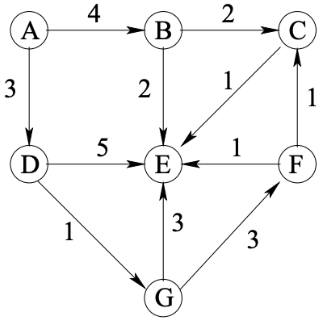
\includegraphics[width=\columnwidth]{djikstra.png}
        \begin{tabular}{ccccccc}
            A: 0          & D: 3          & B: 4          & G: 4          & C: 6
                          & E: 6          & F: 7                                 \\
            B: \(\infty\) & B: 4          & G: 4          & C: 6          & E: 6
                          & F: 7                                                 \\
            C: \(\infty\) & C: \(\infty\) & E: 8          & E:6           & F: 7
            \\
            D: \(\infty\) & E: \(\infty\) & C: \(\infty\) & F: \(\infty\)
            \\
            E: \(\infty\) & F: \(\infty\) & F: \(\infty\)
            \\
            F: \(\infty\) & G: \(\infty\)
            \\
            G: \(\infty\)
        \end{tabular}

    \end{multicols*}
    \columnbreak
    \subsection*{Floyd-Warshall}
    Let \(d_{ij}^{(k)}\) be the weight of the shortest path from \(i\) to \(j\)
    with all intermediate vertices in the set \(\{1, 2, \ldots, k\}\).

    % \vspace*{-1em}
    \begin{equation*}
        d_{ij}^{(k)} = \begin{cases}
            w_{ij}                                                & \text{if } k = 0 \\
            \min(d_{ij}^{(k-1)}, d_{ik}^{(k-1)} + d_{kj}^{(k-1)}) & \text{if } k > 0 \\
        \end{cases}
    \end{equation*}

    \begin{center}
        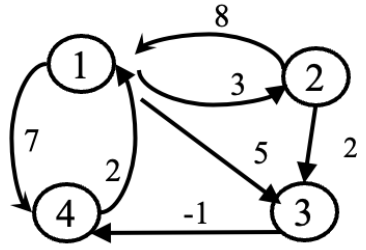
\includegraphics[width=0.65\columnwidth]{floyd.png}
    \end{center}
    \begin{align*}
        D^0 & = \begin{array}{c|cccc}
                      & 1      & 2      & 3      & 4      \\
                    \hline
                    1 & 0      & 3      & 5      & 7      \\
                    2 & 8      & 0      & 2      & \infty \\
                    3 & \infty & \infty & 0      & -1     \\
                    4 & 2      & \infty & \infty & 0
                \end{array}
            & P = \begin{array}{c|cccc}
                        & 1 & 2 & 3 & 4 \\
                      \hline
                      1 & 0 & 0 & 0 & 0 \\
                      2 & 0 & 0 & 0 & 0 \\
                      3 & 0 & 0 & 0 & 0 \\
                      4 & 0 & 0 & 0 & 0
                  \end{array}                \\
        D^1 & = \begin{array}{c|cccc}
                      & 1      & 2      & 3 & 4  \\
                    \hline
                    1 & 0      & 3      & 5 & 7  \\
                    2 & 8      & 0      & 2 & 15 \\
                    3 & \infty & \infty & 0 & -1 \\
                    4 & 2      & 5      & 7 & 0
                \end{array}
            & P = \begin{array}{c|cccc}
                        & 1 & 2 & 3 & 4 \\
                      \hline
                      1 & 0 & 0 & 0 & 0 \\
                      2 & 0 & 0 & 0 & 1 \\
                      3 & 0 & 0 & 0 & 0 \\
                      4 & 0 & 1 & 1 & 0
                  \end{array}                \\
        D^2 & = \begin{array}{c|cccc}
                      & 1      & 2      & 3 & 4  \\
                    \hline
                    1 & 0      & 3      & 5 & 7  \\
                    2 & 8      & 0      & 2 & 15 \\
                    3 & \infty & \infty & 0 & -1 \\
                    4 & 2      & 5      & 7 & 0
                \end{array}
            & P = \begin{array}{c|cccc}
                        & 1 & 2 & 3 & 4 \\
                      \hline
                      1 & 0 & 0 & 0 & 0 \\
                      2 & 0 & 0 & 0 & 1 \\
                      3 & 0 & 0 & 0 & 0 \\
                      4 & 0 & 1 & 1 & 0
                  \end{array}                \\
        D^3 & = \begin{array}{c|cccc}
                      & 1      & 2      & 3 & 4  \\
                    \hline
                    1 & 0      & 3      & 5 & 4  \\
                    2 & 8      & 0      & 2 & 1  \\
                    3 & \infty & \infty & 0 & -1 \\
                    4 & 2      & 5      & 7 & 0
                \end{array}
            & P = \begin{array}{c|cccc}
                        & 1 & 2 & 3 & 4 \\
                      \hline
                      1 & 0 & 0 & 0 & 3 \\
                      2 & 0 & 0 & 0 & 3 \\
                      3 & 0 & 0 & 0 & 0 \\
                      4 & 0 & 1 & 1 & 0
                  \end{array}                \\
        D^4 & = \begin{array}{c|cccc}
                      & 1 & 2 & 3 & 4  \\
                    \hline
                    1 & 0 & 3 & 5 & 4  \\
                    2 & 3 & 0 & 2 & 1  \\
                    3 & 1 & 4 & 0 & -1 \\
                    4 & 2 & 5 & 7 & 0
                \end{array}
            & P = \begin{array}{c|cccc}
                        & 1 & 2 & 3 & 4 \\
                      \hline
                      1 & 0 & 0 & 0 & 3 \\
                      2 & 4 & 0 & 0 & 3 \\
                      3 & 4 & 4 & 0 & 0 \\
                      4 & 0 & 1 & 1 & 0
                  \end{array}
    \end{align*}


    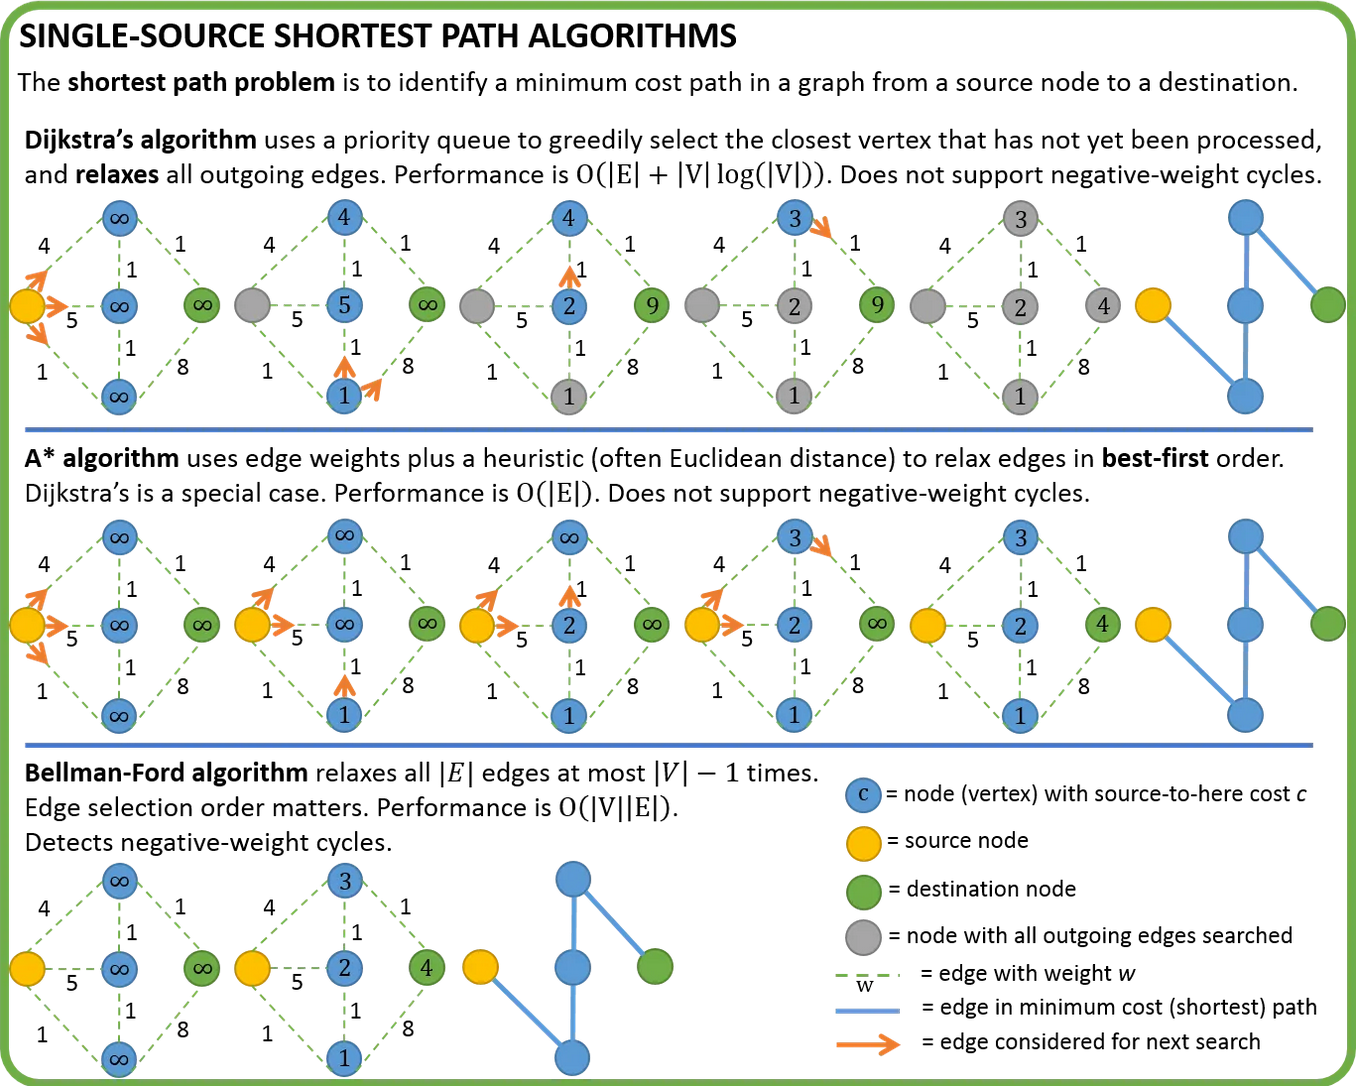
\includegraphics[width=\linewidth]{paths.png}
    \subsection*{Knapsack}
    \begin{equation*}
        c[i, w] = \begin{cases}
            0                                    & \text{if } i = 0 \text{ or } w = 0 \\
            c[i-1, w]                            & \text{if } w_i > w                 \\
            \max(c[i-1, w], c[i-1, w-w_i] + v_i) & \text{otherwise}
        \end{cases}
    \end{equation*}

    \section*{Bellman-Ford}
    Bellman-Ford is a single source shortest path algorithm that determines the
    shortest path between a given source vertex and every other vertex in a
    graph. This algorithm can be used on both weighted and unweighted graphs.

    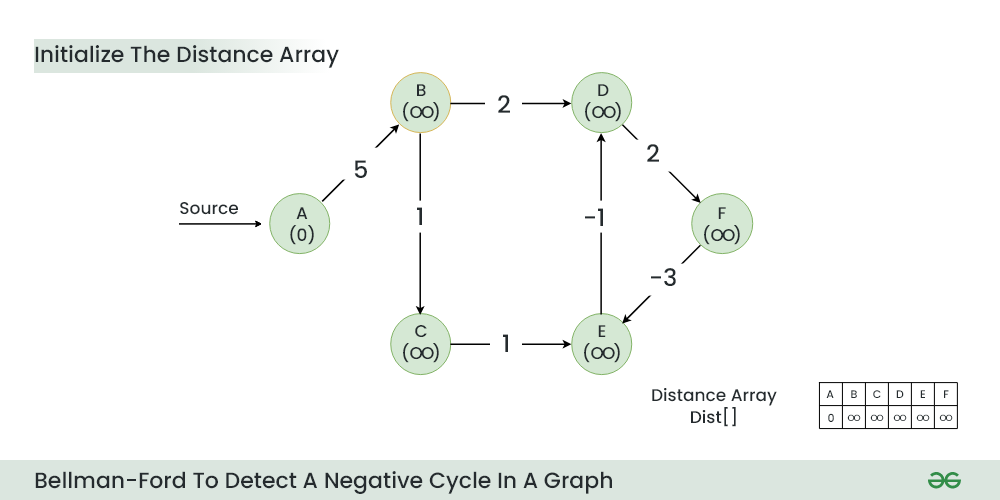
\includegraphics[width=\linewidth]{bellman.png}

    \begin{multicols*}{2}
        % \begin{enumerate}
        %     \item Initialize distance array to store shortest dist for each
        %           vertex. Initialize source as 0, and all others to be
        %           \(\infty\).
        %     \item Relax all edges \(|V| - 1\) times.
        %     \item Relax all edges one more time to detect negative cycles.
        % \end{enumerate}
        \begin{description}
            \item[Base Case] \(\ell_{ss}^{(0)} = 0; \ell_{sv}^{(0)} = \infty\)
            \item[Recurrence] \[\ell_{sv}^{(k)} = \min_{u \in V} \left\{ \ell_{su}^{(k-1)} + w_{uv} \right\}\]
            \item[Optimal] \[\ell_{sv}^{|V|-1} \text{ for all } v \in V\]
        \end{description}
        \begin{equation*}
            w_ij = \begin{cases}
                0,       & i = j                                 \\
                w(i, j), & i \neq j \text{ and } (i, j) \in E    \\
                \infty,  & i \neq j \text{ and } (i, j) \notin E
            \end{cases}
        \end{equation*}
        \begin{align*}
            \begin{array}{|c|c|c|c|c|c|}
                \hline
                A & B      & C      & D      & E      & F      \\
                \hline
                0 & \infty & \infty & \infty & \infty & \infty \\
                \hline
                0 & 5      & \infty & \infty & \infty & \infty \\
                \hline
                0 & 5      & 6      & 7      & \infty & \infty \\
                \hline
                0 & 5      & 6      & 7      & 7      & 9      \\
                \hline
                0 & 5      & 6      & 6      & 6      & 9      \\
                \hline
                0 & 5      & 6      & 5      & 6      & 8      \\
                \hline
            \end{array}
        \end{align*}
    \end{multicols*}
    \setlength{\leftmargini}{8em}
    \footnotesize
    \begin{enumerate}[label=Relaxation \arabic*:]
        \item \begin{align*} Dist(B) & > Dist(A) + w(A, B)             \\
               \infty  & > 0 + 5 \Rightarrow Dist(B) = 5
              \end{align*}
        \item \begin{align*} Dist(D) > Dist(B) + w(B, D) \\
                  \infty > 5 + 2 \Rightarrow Dist(D) = 7
              \end{align*}
              \begin{align*}
                  Dist(C) > Dist(B) + w(B, C) \\
                  \infty > 5 + 1 \Rightarrow Dist(C) = 6
              \end{align*}
        \item \begin{align*} Dist(F) > Dist(D) + w(D, F) \\
                  \infty > 7 + 2 \Rightarrow Dist(F) = 9
              \end{align*}
              \begin{align*}
                  Dist(E) > Dist(C) + w(C, E) \\
                  \infty > 6 + 1 \Rightarrow Dist(E) = 7
              \end{align*}
        \item \begin{align*} Dist(D) > Dist(E) + w(E, D) \\
                  7 > 7 + (-1) \Rightarrow Dist(D) = 6
              \end{align*}
              \begin{align*}
                  Dist(E) > Dist(F) + w(F, E) \\
                  7 > 9 + (-3) \Rightarrow Dist(E) = 6
              \end{align*}
        \item \begin{align*} Dist(F) > Dist(D) + w(D, F) \\
                  9 > 6 + 2 \Rightarrow Dist(F) = 8
              \end{align*}
              \begin{align*}
                  Dist(D) > Dist(E) + w(E, D) \\
                  6 > 6 + (-1) \Rightarrow Dist(D) = 6
              \end{align*}
        \item \begin{align*} Dist(E) > Dist(F) + w(F, E) \\
                  6 > 8 + (-3) \Rightarrow Dist(E) = 5
              \end{align*}
              \begin{align*}
                  Dist(F) > Dist(D) + w(D, F) \\
                  8 > 5 + 2 \Rightarrow Dist(F) = 7
              \end{align*}
    \end{enumerate}
    \small
    \subsection*{Network Flow}
    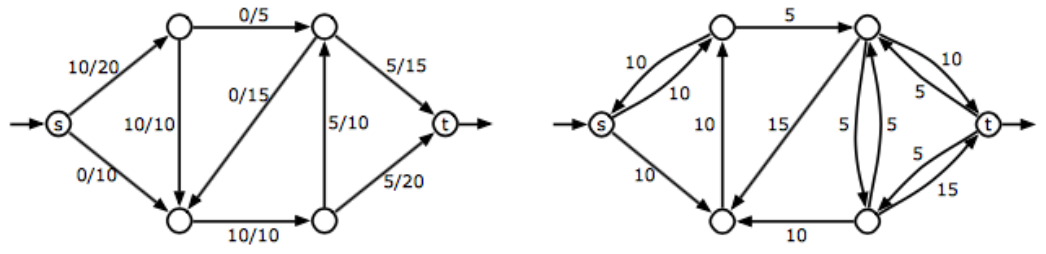
\includegraphics[width=\linewidth]{residual.png}
    \begin{description}
        \item[Flow] Amount of material that can be transported between two
            nodes.
        \item[Capacity] Maximum amount of material that can be transported
            between two nodes.
        \item[Residual Capacity] Amount of material that can still be
            transported between two nodes.
        \item[Augmenting Path] Path from source to sink where all edges have
            residual capacity.
        \item[Residual Graph] Graph where edges have residual capacity.
    \end{description}

    \begin{multicols*}{2}
        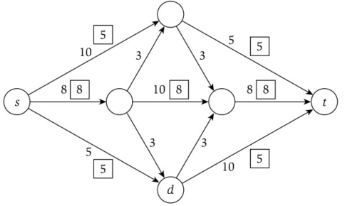
\includegraphics[width=\linewidth]{residual1.png}
        % \columnbreak
        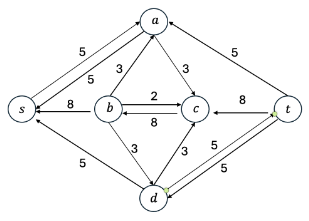
\includegraphics[width=\linewidth]{residual2.png}
    \end{multicols*}


    \subsection*{Dyanmic Programming}
    \begin{enumerate}
        \item Characterize structure of an optimal solution.
        \item Recursively define value of an optimal solution.
        \item Compute the value in a bottom-up fashion.
        \item Construct an optimal solution from computed information.
    \end{enumerate}
    \subsubsection*{1D Example}
    Let \(D_n\) be the number of ways to write \(n\) as the sum of 1, 3, and 4.
    Find the recurrence:
    \begin{enumerate}
        \item Consider one possible solution, \(n = x_1 + x_2 + \dots + x_m\)
        \item If \(x_m = 1\), rest of the terms must sum to \(n - 1\)
        \item Thus, number of sums that end with \(x_m = 1\) is \(D_{n-1}\)
        \item Take other cases into account \((x_m = 3, x_m = 4)\)
    \end{enumerate}
    \begin{equation*}
        D_n = D_{n-1} + D_{n-3} + D_{n-4}
    \end{equation*}

    \subsubsection*{Rod Cutting}
    \begin{itemize}
        \item Has optimal sub-structure property (must have optimal cut for each
              sub-problem to get global optimal)
        \item Has recursive exponential solution
        \item Has polynomial DP solution
    \end{itemize}

    \subsection*{Greedy Algorithm}
    \begin{description}
        \item[Optimal Substructure] The optimal solution to a problem
            incorporates the optimal solution to subproblems.
        \item[Greedy Choice Property] Locally optimal choice leads to globally
            optimal solution.
        \item[Overlapping Subproblems] Subproblems recur many times.
    \end{description}

    \setlength{\leftmargini}{0em}
    \setlength{\columnsep}{2em}

    \begin{multicols*}{2}
        \subsubsection*{DP}
        \begin{itemize}
            \item Used to solve optimization
            \item Has \textbf{optimal substructure}
            \item Make an `informed choice' after getting optimal solutions to subproblems
            \item Bottom-up
            \item Dependent on overlapping subproblems
        \end{itemize}
        % \columnbreak
        \subsubsection*{Greedy}
        \begin{itemize}
            \item Used to solve optimization
            \item Has \textbf{optimal substructure}
            \item Make a `greedy choice' before solving subproblem
            \item Top-down
                  \begin{itemize}
                      \item Each round selects only one subproblem
                      \item Subproblem size decreases
                  \end{itemize}
            \item No overlapping subproblems
        \end{itemize}
    \end{multicols*}

    \subsection*{DFS Applications}
    \begin{itemize}
        \item Finding connected components on an undirected graph
        \item Detecting cycles on a graph
        \item Topological sorting on a directed acyclic graph (DAG)
        \item Finding strongly connected components (SCC) in a directed graph
    \end{itemize}
    \emph{Lemma:} A directed graph is acylic iff a DFS of the graph yields no back edges.

    \subsubsection*{Strongly Connected Components}
    The SCC of a directed graph are the \emph{equivalence classes of verticies}
    under the `mutually reachable' relation. That is, a SCC is a maximal subset
    of mutually reachable nodes.

    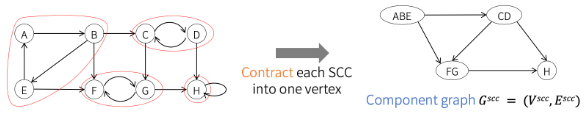
\includegraphics[width=\columnwidth]{scc.png}

    \subsubsection*{Spanning Tree}
    Spanning tree of an undirected graph is a tree that connects all verticies.
    \setlength{\columnsep}{-8em}
    \begin{multicols*}{2}
        \begin{itemize}
            \item Exactly \(|V| - 1\) edges
            \item Acyclic
            \item Non-unique
        \end{itemize}
        \subsubsection*{Minimum Spanning Tree}
        \begin{description}
            \item[Kruskal] Consider edges in ascending order of weight. Each
                step, select next edge as long as it doesn't make a cycle.
            \item[Prim] Start with any vertex and grow a tree from it. At each
                step, add edge of the least weight to connect an isolated vertex.
        \end{description}
    \end{multicols*}
    MST is unique if all edge weights are distinct.

    \subsection*{String Matching}
    \subsubsection*{Rabin-Karp}
    Compare a string's hash values.
    \subsubsection*{Knuth-Morris-Pratt}
    \begin{itemize}
        \item Linear time for exact matching
        \item Compares left to right, shifts more than one position
        \item Preprocessing approach to avoid trivial comparisons
        \item Conceived by Donald Knuth and Vaughan Pratt
        \item Worst-Case \(\Theta((n - m + 1) m)\)
    \end{itemize}
    \texttt{ABABCABCABAABABD}
    LPS=[0, 0, 1, 2, 0]


    \subsection*{Complexity Theory}
    \setlength{\columnsep}{0em}
    \begin{multicols*}{2}
        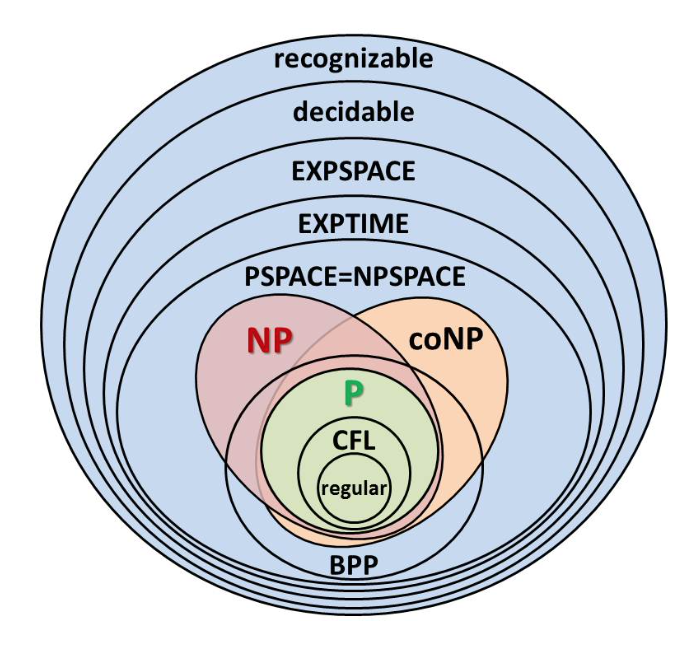
\includegraphics[width=\columnwidth]{complexity.png}
        \columnbreak
        \begin{description}
            \item[NP] Verifiable in polynomial time
            \item[P] Solvable in polynomial time
            \item[NP-Hard] At least as hard has all NP problems
            \item[NP-Complete] Both NP and NP-Hard
        \end{description}
    \end{multicols*}
\end{multicols*}
\subsection*{Psuedocodes}
\lstset{basicstyle=\footnotesize}
\begin{lstlisting}
Optimal-BST(p, q, n)
    let e[1..n + 1, 0..n], w[1..n + 1, 0..n], and root[1..n, 1..n] be new tables
    for i = 1 to n + 1
        e[i, i - 1] = 0
        w[i, i - 1] = 0
    for l = 1 to n
        for i = 1 to n - l + 1
            j = i + l - 1
            e[i, j] = infty
            w[i, j] = w[i, j - 1] + p[j]
            for r = i to j
                t = e[i, r - 1] + e[r + 1, j] + w[i, j]
                if t < e[i, j]
                    e[i, j] = t
                    root[i, j] = r
    return e and root
\end{lstlisting}

\begin{multicols*}{2}


    \begin{lstlisting}[language=java]
floydWarshall(int dist[][])
for k=0 to V
    for i=0 to V
        for j=0 to V
            if (dist[i][k] + dist[k][j] < dist[i][j])
                dist[i][j] = dist[i][k] + dist[k][j]
\end{lstlisting}

    \begin{lstlisting}
LCS-Length(X, Y, m, n)
    let b[1..m, 1..n] and c[0..m, 0.. n] be new tables
    for i = 0 to m
        c[i, 0] = 0
    for j = 0 to n
        c[0, j] = 0
    for i = 1 to m
        for j = 1 to n
            if x[i] == y[j]
                c[i, j] = c[i - 1, j - 1] + 1
                b[i, j] = "NW"
            else if c[i - 1, j] >= c[i, j - 1]
                c[i, j] = c[i - 1, j]
                b[i, j] = "N"
            else
                c[i,j] = c[i, j - 1]
                b[i, j] = "W"
    return c and b
\end{lstlisting}


    \begin{lstlisting}
DFS(G)
    for each vertex u in G.V
        u.color = WHITE
        u.pi = NIL
    time = 0
    for each vertex u in G.V
        if u.color == WHITE
            DFS-Visit(G, u)

DFS-Visit(G, u)
    time = time + 1
    u.d = time
    u.color = GRAY
    for each v in G.Adj[u]
        if v.color == WHITE
            v.pi = u
            DFS-Visit(G, v)
    u.color = BLACK
    time = time + 1
    u.f = time
\end{lstlisting}

    \begin{lstlisting}
KMP-Matcher(T, P)
    n = T.length
    m = P.length
    pi = Compute-Prefix-Function(P)
    q = 0
    for i = 1 to n
        while q > 0 and P[q + 1] != T[i]
            q = pi[q]
        if P[q + 1] == T[i]
            q = q + 1
        if q == m
            print "Pattern occurs with shift" i - m
            q = pi[q]
    \end{lstlisting}
    \columnbreak
    \vspace*{-12em}
    \begin{lstlisting}
Compute-Prefix-Function(P)
    n = P.length
    let pi[0..n] be a new table
    for i = 0 to n
        j = pi[i - 1]
        while j > 0 and P[i] != P[j]
            j = pi[j - 1]
        if P[i] == P[j]
            j = j + 1
        pi[i] = j
    return pi
\end{lstlisting}

    \lstset{language=python}
    \begin{lstlisting}
def knapsack(W, wt, val, n):
dp = [[0] * (W+1) for _ in range(n+1)]

for i in range(1, n+1):
    for w in range(1, W+1):
        if wt[i-1] <= w:
            dp[i][w] = max(val[i-1] + dp[i-1][w-wt[i-1]],
                dp[i-1][w])
        else:
            dp[i][w] = dp[i-1][w]

return dp[n][W]
\end{lstlisting}

    \begin{lstlisting}
def edit_distance(s1, s2):
m, n = len(s1), len(s2)
dp = [[0] * (n+1) for _ in range(m+1)]

for i in range(m+1):
    for j in range(n+1):
        if i == 0:
            dp[i][j] = j
        elif j == 0:
            dp[i][j] = i
        elif s1[i-1] == s2[j-1]:
            dp[i][j] = dp[i-1][j-1]
        else:
            dp[i][j] = 1 + min(dp[i-1][j],
                dp[i][j-1], dp[i-1][j-1])

return dp[m][n]
\end{lstlisting}

    \begin{lstlisting}
def coin_change(coins, amount):
dp = [float('inf')] * (amount+1)
dp[0] = 0

for i in range(1, amount+1):
    for coin in coins:
        if coin <= i:
            dp[i] = min(dp[i], dp[i-coin] + 1)

return dp[amount] if dp[amount] != float('inf') else -1
\end{lstlisting}

    \begin{lstlisting}
def tsp(graph, start):
n = len(graph)
visited = (1 << n) - 1
memo = {}

def dfs(node, visited):
    if visited == 0:
        return graph[node][start]

    if (node, visited) in memo:
        return memo[(node, visited)]

    ans = float('inf')
    for i in range(n):
        if visited & (1 << i):
            ans = min(ans, graph[node][i] +
                dfs(i, visited ^ (1 << i)))

    memo[(node, visited)] = ans
    return ans

return dfs(start, visited)
\end{lstlisting}

\end{multicols*}
\end{document}